\documentclass[a4paper, 12pt]{report}
\usepackage{graphicx}
\usepackage[french]{babel}
\usepackage{caption}
\usepackage[utf8]{inputenc}
\usepackage[T1]{fontenc}
\usepackage{multirow}
\usepackage{listings}
\usepackage{float}
\usepackage{url}
\usepackage[french]{algorithm}
\usepackage{style/myalgorithm}
\usepackage{amsmath,amsfonts,amssymb}
\newcommand{\fBm}{\emph{fBm}~}
\newcommand{\etal}{\emph{et al.}~}
\newcommand{\glAd}{\emph{GL4D}~}
\newcommand{\apiopengl}{API OpenGL\textsuperscript{\textregistered}~}
\newcommand{\opengl}{OpenGL\textsuperscript{\textregistered}~}
\newcommand{\opengles}{OpenGL\textsuperscript{\textregistered}ES~}
\newcommand{\clang}{langage \texttt{C}}
\newcommand{\codesource}{\textsc{Code source}~}
\floatstyle{ruled}
\newfloat{programslist}{htbp}{locs}
\newcommand{\listofprograms}{\listof{programslist}{Liste des codes source}}
\newcounter{program}[subsection]
\renewcommand{\theprogram}{\arabic{chapter}.\arabic{program}}

\newenvironment{program}[1]{
  \if\relax\detokenize{#1}\relax
  \gdef\mycaption{\relax}
  \else
  \gdef\mycaption{#1}
  \fi
  \refstepcounter{program}
  \addcontentsline{locs}{section}{#1}
  \footnotesize
}{
  \begin{description}
    \item[\codesource \theprogram]--~\mycaption
  \end{description}
}

\begin{document}
\begin{titlepage}
  \begin{center}
    \begin{tabular*}{\textwidth}{l@{\extracolsep{\fill}}r}
      \includegraphics[height=1.5cm]{images/m2ise.png}
    \end{tabular*}
    \small 
    \rule{\textwidth}{.5pt}~\\
    \large 
    \textsc{Université Paris 8 - Vincennes à Saint-Denis}\vspace{0.5cm}\\
    \textbf{Master Informatique des Systèmes Embarqués}\vspace{3.0cm}\\
    \Large
    \textbf{Memoire de projet tuteuré}\vspace{1.5cm}\\
    \large
    \textbf{Fakhri \textsc{YAHIAOUI} - Roman \textsc{BOURSIER}}\vspace{1.5cm}\\
    Date de soutenance : le 09/06/2020\vspace{1.75cm}\\
  \end{center}\vspace{1.5cm}~\\
  \begin{tabular}{ll}
    \hspace{-0.45cm}Tuteur -- Université~:~&~Farès \textsc{BELHADJ}\\
  \end{tabular}
\end{titlepage}
\chapter*{Résumé}
\markboth{\sc Résumé}{}
\addcontentsline{toc}{chapter}{Résumé} 

Le présent document présente notre travail effectué dans la cadre de notre mémoire de fin d'étude.

Dans un premier temps, nous présentons le projet et son contexte, puis nous abordons les différentes solutions existantes à travers la section "état de l'art". Nous exposons ensuite nos propositions de solutions et leurs évaluations respectives. En conclusions nous faisons le bilan de ce travail ainsi que les points d'améliorationd possibles de nos modèles.

%% Table des matières
\tableofcontents

\chapter*{Introduction}
\markboth{\sc Introduction}{}
\addcontentsline{toc}{chapter}{Introduction}

Nous souhaitons utiliser un modèle de Deep Learning, afin de produire un moteur de rendu capable d’adopter une stylisation « type » tel que la peinture chinoise. Dans un premier temps, il s’agira de proposer un modèle d’abstraction des peintures sélectionnées comme base d’apprentissage et d’utiliser le couple « peinture originale » / « abstraction » pour l’entraînement. Par la suite, un moteur de rendu d’abstractions sera connecté au réseau profond qui produira une peinture sur la base de l’abstraction.

Le modèle généré devra d'une part adopter la stylisation retenue mais aussi interpréter l'abstraction d'origine.

\section{Contexte}

La "traduction image-image" (Image-to-image translation) permet d'apprendre le mapping entre une image d'entrée et de sortie. En figure \ref{fig-pix2pix}, nous testons la génération d'un paysage à partir d'un croquis simple. En figure \ref{fig-pix2pix-fail}, c'est un échec.

\begin{center}
\includegraphics[width=0.7\linewidth]{images/pix2pix-t1.png}
\captionof{figure}{Test du framework pix2pix \cite{DBLP:journals/corr/IsolaZZE16} sur notre dataset composé de photos de paysages, labellisées en appliquant un filtre Canny \cite{4767851} sur chacune d'elles.}
\label{fig-pix2pix}
\end{center}

\begin{center}
\includegraphics[width=0.7\linewidth]{images/pix2pix-fail.png}
\captionof{figure}{Utilisation du même modèle avec une abstraction d'arbre}
\label{fig-pix2pix-fail}
\end{center}

Comme évoqué dans \cite{DBLP:journals/corr/abs-1805-00247} les algorithmes du type "traduction image-image" se basent essentiellement sur la corrélation d'une image à l'autre, et relève d'un apprentissage supervisé. Le rendu en figure \ref{fig-pix2pix-fail} s'explique par la nature du dataset et par la distance importante qui sépare une abstraction d'une photo. 

En figure \ref{fig-croquis} nous avons demandé à plusieurs personnes de dessiner un paysage composé de montagnes et d'arbres, éléments courants de la peinture chinoise. Ces dessins sont des abstractions, que nous souhaitons traduire en peintures chinoises.

\begin{center}
  \centering
  \begin{tabular}{ccc}
    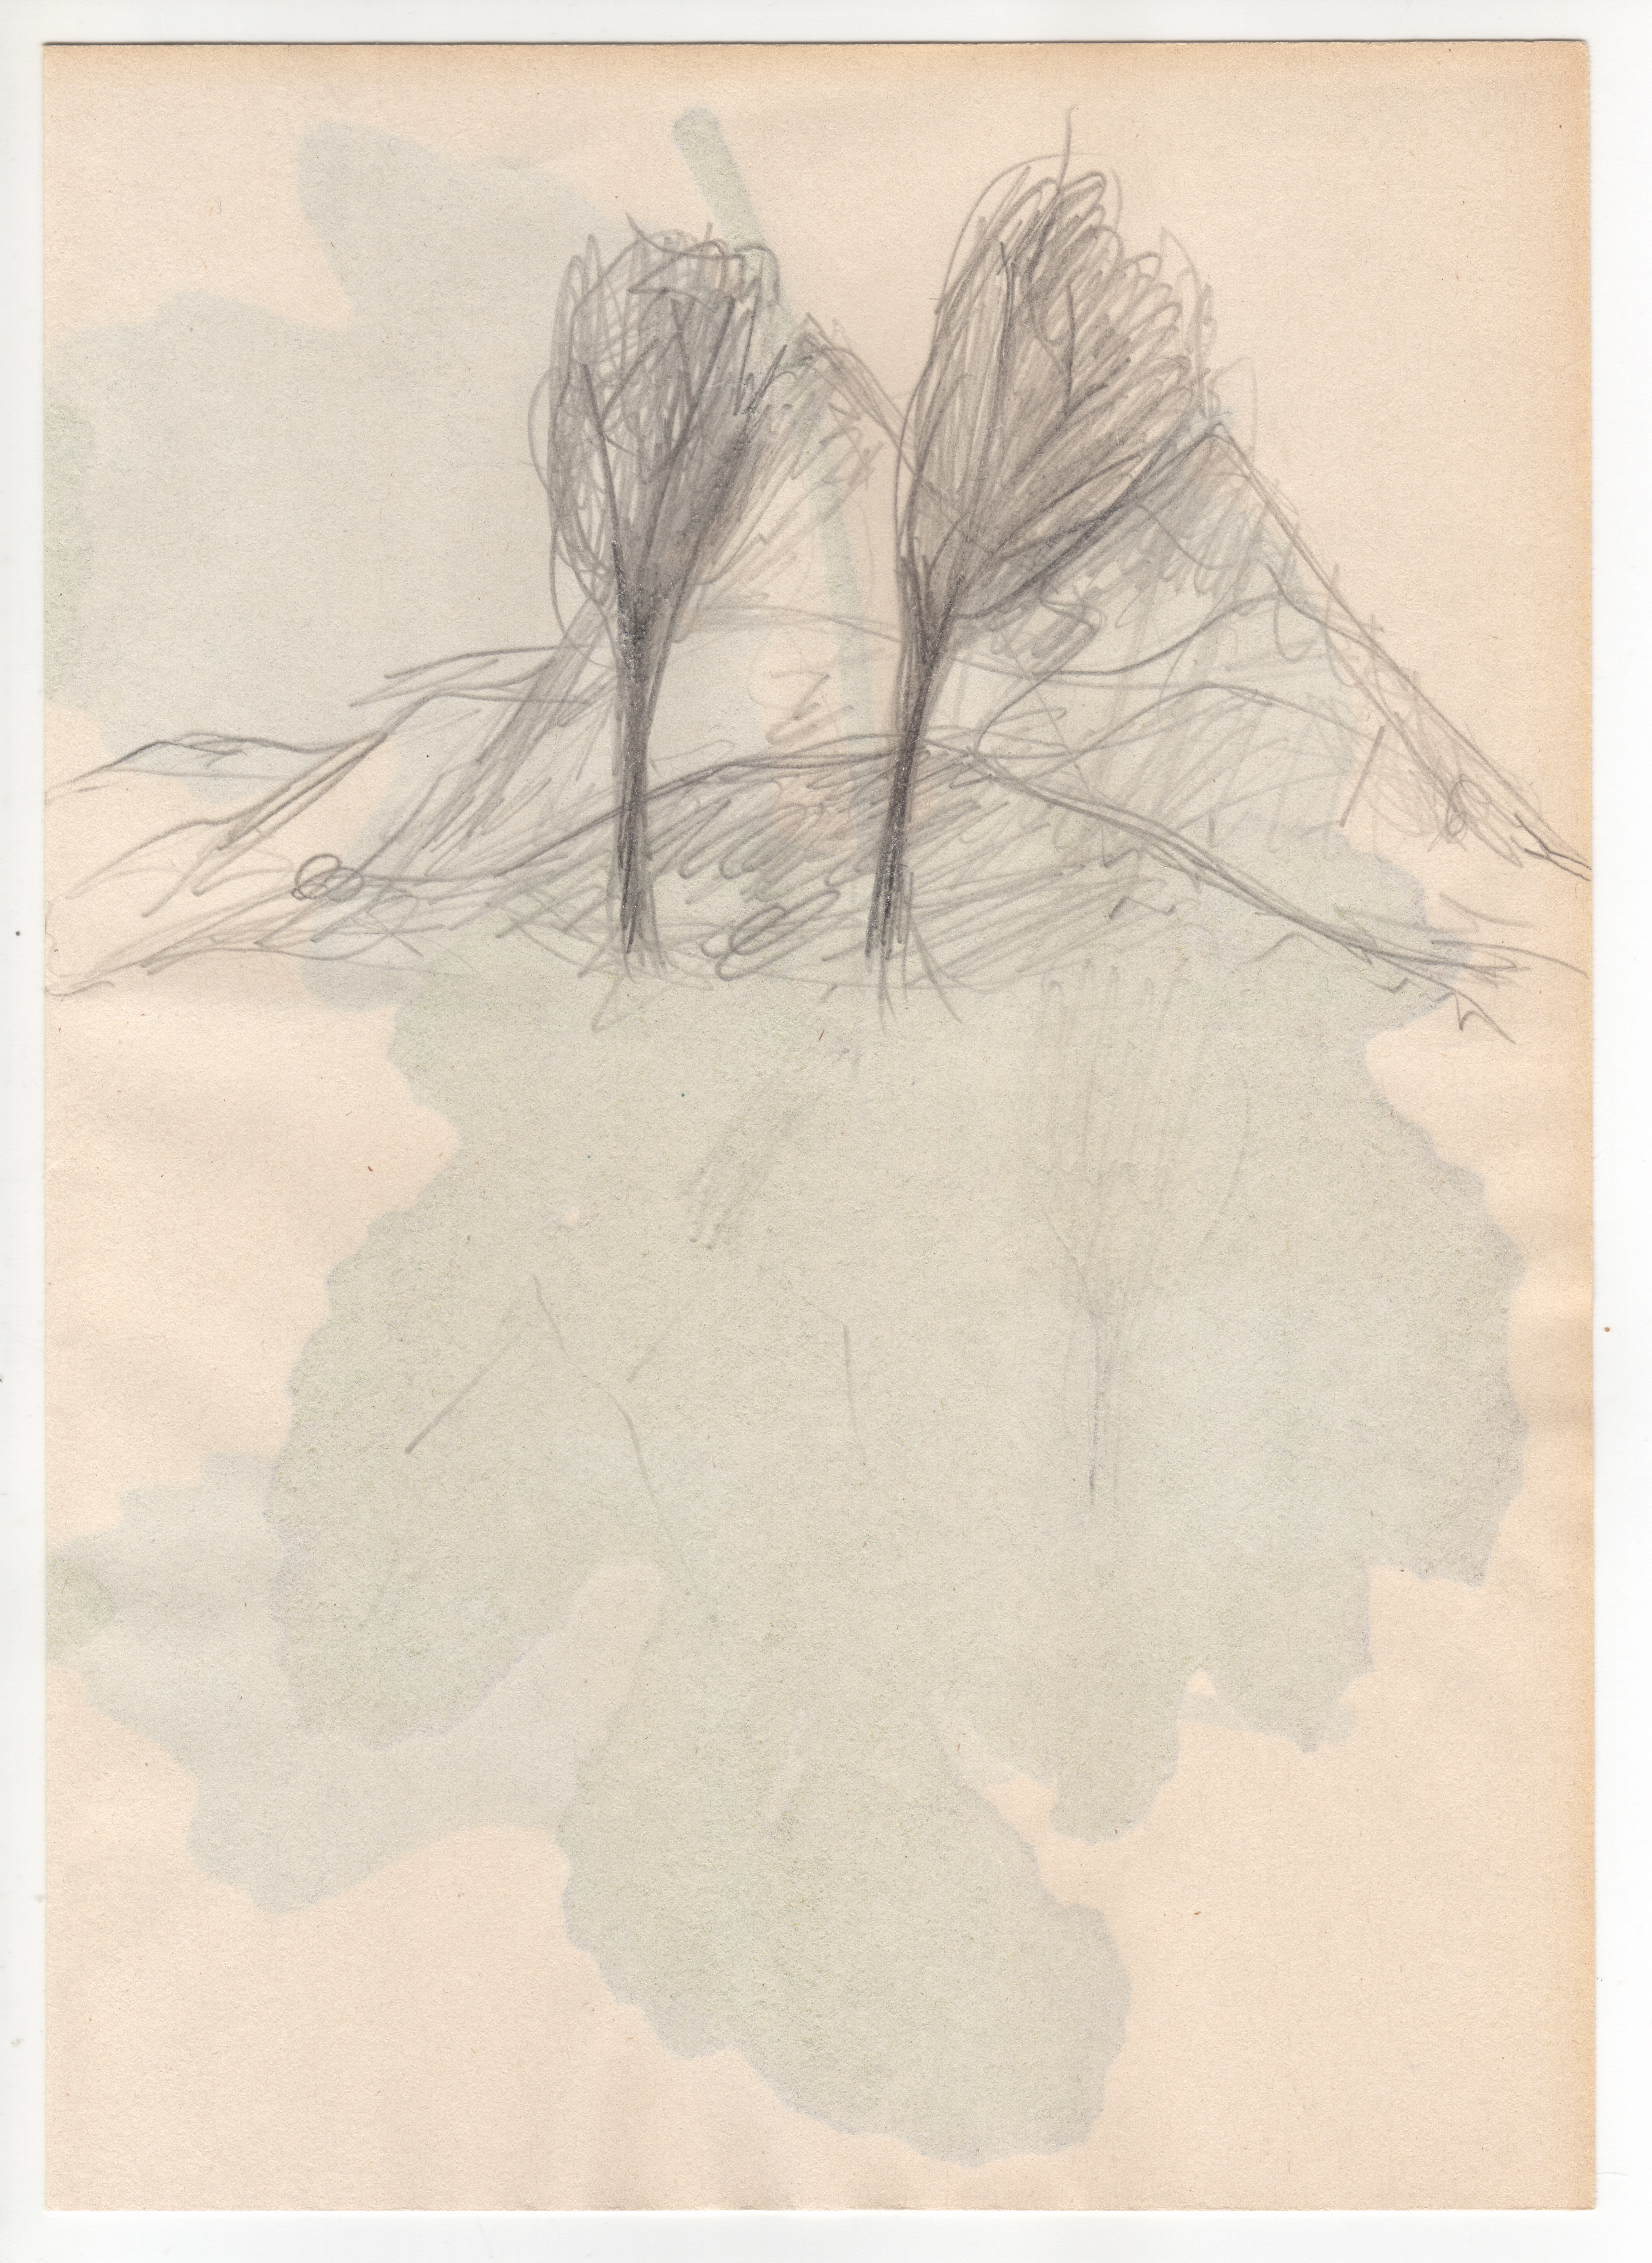
\includegraphics[angle=90, height=0.15\textheight]{images/croquis_1.jpg}&
    \includegraphics[angle=90, height=0.15\textheight]{images/croquis_2.jpg}&
    \includegraphics[angle=90, height=0.15\textheight]{images/croquis_4.jpg}\\
    (a)&(b)&(c)
  \end{tabular}
  \captionof{figure}{Dessin de paysages réalisés par des personnes différentes. On note que les niveaux d'informations sont plus ou moins élevés. Le dessin (b) est très abstrait tandis que nous observons plus de détails pour (a) .\label{fig-croquis}}
\end{center}



\chapter{Etat de l'art}
 
Nous présentons dans un premier temps les GANs qui sont au coeur de notre problématique. En un second lieu, nous étudions différents modèles existants basés sur les GANs conditionnels. 

\section{Généralités sur les GANs}

"Les GANs (en anglais generative adversarial networks) sont une classe d'algorithmes d'apprentissage non-supervisé. Ces algorithmes ont été introduits dès 2014 par Goodfellow et permettent de générer des images avec un fort degré de réalisme." \cite{wiki:Reseaux-antagonistes-generatifs}

Un générateur fabrique des données et les soumet au discriminateur dont le but est d'évaluer leurs degrés de crédibilité. 

Le générateur $G(z, \theta_{1})$ représente un réseau de neurones capable de mapper du bruit $z$ vers l'espace désiré $x$. Le discriminateur $D(z, \theta_{2})$ retourne la probabilité dans l'intervalle $[0,1]$ que $x$ vient du dataset original. $\theta_{i}$ représente les poids définis par chacun des modèles. Le générateur tente de maximiser la probabilité que les données $x$, soient classifiées comme appartenant au dataset d'origine et inversement, le discriminateur minimise la probabilité que de fausses images appartiennent au dataset d'origine.

Il existe aujourd'hui une très grande variété de travaux de recherches basés sur les GANs (BCGAN, AmbientGAN, ORGAN, Perceptual GAN). Le dépôt "The GANs Zoo" \cite{hindupuravinash} référençait déjà en 2018 plus de 502 noms de GANs différents !


\section{CGANs et traduction d'image}

Les GANs conditionnels ajoutent une information supplémentaire $y$, partagée par le discriminateur et le générateur. Grâce aux cGANs il est possible de générer des images réalistes basées sur des labels de classes, des textes ou des images.

\subsection{Pix2Pix}
\cite{DBLP:journals/corr/GatysEB15a} nous montre en quoi les cGANs peuvent permettre de résoudre efficacement les problèmes de traductions d'images et propose un framework applicable à n'importe quel domaine.

\subsection{GauGan}
\cite{DBLP:journals/corr/abs-1903-07291} permet de générer des paysages réalistes basés sur des masques de segmentation sémantiques. Les auteurs introduisent la "normalisation conditionnel" ou "adaptative", permettant de prendre en compte notamment les informations spatiales.
Les couches de normalisations ont tendance à faire perdre de l'information contenu dans les masques sémantiques d'entrées car ils ne dépendent pas de données externes.

\begin{center}
  \centering
  \begin{tabular}{cc}
    \includegraphics[height=0.15\textheight]{images/test-gaugan-sm.jpg}&
    \includegraphics[height=0.15\textheight]{images/test-gaugan.jpg}\\
    (a) Input - masques de segmentation sémantiques &(b) Output
  \end{tabular}
  \captionof{figure}{Test de rendu de paysage à partir de l'application Gaugan : http://nvidia-research-mingyuliu.com/gaugan/\label{fig-gaugan}}
\end{center}

\subsection{CycleGan}
CycleGan \cite{CycleGAN2017}, présente une approche pour la traduction d'une image d'un domaine source vers un domaine cible lorsque le dataset n'est pas apparié. \\

Le modèle possède deux générateurs $G:X\to Y$ et un second $F:Y\to X$ ainsi que deux discriminateurs $D_Y$ and $D_X$

Les auteurs nous expliquent que si nous pouvons passer du domaine $X$ vers le domaine $Y$ et vice-versa, alors le résultat final devrait être identique à l'entrée initiale $X$.

\subsection{Transfert de style neuronal} 
Introduit par Leon A. Gatys \cite{DBLP:journals/corr/GatysEB15a} le TDN consiste à transférer un style à partir d'une image de référence vers une image de contenu. L'objectif est de transformer l'image d'entrée (bruit) en minimisant la distance avec l'image de contenu et avec l'image de style. On obtient alors par rétropropagation, une image qui correspond au contenu de l'image d'origine et au style souhaitée.

L'avantage de cette technique est qu'elle ne nécessite pas de dataset, seules deux images sont nécessaires.

\begin{center}
  \centering
  \begin{tabular}{ccc}
    \includegraphics[height=0.15\textheight]{images/test-gaugan.jpg}&
    \includegraphics[height=0.15\textheight]{images/transfert-ds.jpg}&
    \includegraphics[height=0.15\textheight]{images/gaugan-tds.jpg}\\
    (a) Image de contenu & (b) Image de style &(c) Résultat
  \end{tabular}
  \captionof{figure}{Test de transfert de style réalisé à partir de la figure \ref{fig-gaugan}\label{fig-transfert-de-style}(b)}
\end{center}


\subsection{Learning to Sketch} 
\cite{DBLP:journals/corr/abs-1805-00247} présente une méthode permettant de transformer une photo en croquis, en essayant d'imiter la façon de faire d'un humain. Le modèle est capable de réaliser le croquis séquentiellement, c'est-à-dire trait par trait. Les auteurs proposent de résoudre le problème des styles subjectifs et variés des dessins fait à la main en utilisant un modèle hybride supervisé/non-supervisé. L'objectif étant de palier "au signal de supervision faible et bruyante" induit par l'écart important entre un croquis et sa photo correspondante. \\

L'architecture est décomposé en 4 sous-modèles contenants chacun leurs propres sous-réseaux d'encodeurs et de décodeurs. Deux réseaux supervisés traduisent respectivement une photo en croquis $D(E(photo))\to sketch$ et un croquis en photo $(D(E(sketch))\to photo)$ . Deux autres réseaux non-supervisés se chargent de la reconstruction. $D(E(photo))\to photo$ et $D(E(sketch))\to sketch$  \\


\subsection{Sketching: Inferring Contour Drawings from Images}
\cite{DBLP:journals/corr/abs-1901-00542} propose une nouvelle approche concernant la détection des contours dans une image. L'article montre que les solutions traditionnelles comme Canny \cite{4767851} , captent uniquement les signaux de haute fréquence dans l’image sans la comprendre. Les auteurs ont collecté un dataset de 5000 pairs "croquis humain/photos", crée manuellement via la plateforme de crowdsourcing "Amazon Mechanical Turk". En effet aucun dataset existant ne convenait (nombre d'éléments dans l'image, limites internes manquantes, le contenu non reconnaissable, les zones ombrées vides etc ..).

Ce modèle également du type "traduction image-image", permet d'avoir plusieurs labels différents pour la même photo, donc plusieurs interprétations différentes.

\begin{center}
  \centering
  \begin{tabular}{cc}
    \includegraphics[height=0.15\textheight]{images/sketching-input.jpg}&
    \includegraphics[height=0.15\textheight]{images/sketchy2.png}\\
    (a) Input &(b) Output
  \end{tabular}
  \captionof{figure}{Test du modèle pré-entraîné sur une photo de paysage\label{fig-gaugan}}
\end{center}


\chapter{Résultats}


\section{Généralités}

\subsection{Implémentations}
Nous proposons dans les sections suivantes un ensemble de tests effectués selon des configurations différentes. Nous avons retenu les cGANs et en particulier plusieurs implémentations des cycleGan et de pix2pix.

Chaque étapes de l'apprentissage consiste d’abord à sélectionner un lot d’exemples réels, puis à utiliser le générateur pour générer de faux échantillons correspondants. Le discriminateur est ensuite mis à jour avec le lot d’images réelles, puis de fausses images. Ensuite, le générateur est mis à jour en fournissant les images sources réelles comme entrée et les prédictions de sortie du discriminateur.

Le générateur possède deux scores de pertes ainsi que le score de somme pondérée retourné de l’appel. Ce score pondéré est utilisé pour mettre à jour les poids du modèle.


\subsection{Datasets}
Malgrè nos recherches, nous n'avons pas trouvé de datasets correspondants exactement à nos besoins, c'est-à-dire des paires d'abstractions/peintures chinoises.Pour les croquis, les plus grosses bases existantes sont TU-Berlin \cite{eitz2012hdhso}, Sketchy \cite{sketchy2016} et Quickdraw. Leurs utilisations est délicate car il s'agit le plus souvent d'objets isolés et non appairés à une image réaliste. Pour la peinture chinoise, nous avons récupéré un premier dataset de 5000 images (\cite{ychen93}) et scrappés des plateformes comme google/baidu et pinterest. Chaque dataset est répartie à 90\% pour l'entraînement et 10\% pour les tests. Nous avons ensuite réduit le nombres d'exemples pour des raisons de temps et d'apprentissage trop longs. Chaque image a été par la suite redimensionnée et recadrée au format 256x256.


\subsection{Evaluations}
En général, les modèles GAN ne convergent pas; au lieu de cela, un équilibre est trouvé entre le générateur et les modèles discriminateurs.

\vspace*{\baselineskip}

\begin{lstlisting}
>1, d1[0.505] d2[0.651] g[75.595]
>2, d1[0.479] d2[0.516] g[69.595]
>3, d1[0.621] d2[0.478] g[75.868]
>4, d1[0.478] d2[0.538] g[65.794]
>5, d1[0.415] d2[0.425] g[70.626]
\end{lstlisting}

\vspace*{\baselineskip}

\begin{itemize}
\item d1 : La perte de discrimination sur des exemples réels
\item d2 : La perte de discrimination sur des exemples générés ou faux
\item g : La perte du générateur (moyenne pondérée des pertes liées à l’affrontement de d1 et d2).
\end{itemize}

\vspace*{\baselineskip}

Par conséquent, nous ne pouvons pas juger facilement quand la formation devrait cesser. Nous avons donc enregistrer le modèle et généré des exemples de traductions image-à-image périodiquement pendant la formation. Les rendus peuvent être évalués à la fin de l’analyse et utilisés pour sélectionner un modèle de générateur final basé sur la qualité d’image générée. 



\pagebreak



\section{Abstraction vers peinture}

L'idée ici est de décomposer le passage de l'abstraction à la peinture en deux étapes, c'est à dire de l'abstraction au dessin détaillé puis du dessin détaillé vers la peinture chinoise.

L'entraînement utilise l'architecture pix2pix décrites dans \cite{DBLP:journals/corr/GatysEB15a}, implémentée sous keras 2.4.0.

Le premier dataset de 654 images a été labellisé manuellement, et le second a été obtenu en appliquant l'algorithme de détection de contours nommé "holistically-nested edge detection" \cite{xie2015holisticallynested} sur les peintures chinoises. HED est basé sur un modèle d'apprentissage profond et permet de mieux résoudre l’ambiguïté liée à la détection des contours et des objets. 


\subsection{Evaluation}
\begin{center}
  \centering
    \includegraphics[width=0.9\linewidth]{images/test.png}
  \captionof{figure}{Scores de pertes pendant l’entraînement \ref{fig-gaugan}\label{fig-transfert-de-style}(b)}
\end{center}


\subsection{Resulats}

\vspace*{\baselineskip}

\begin{center}
  \centering
  \begin{tabular}{cc}
    \includegraphics[height=0.2\textheight]{images/abs-input.jpg}&
    \includegraphics[height=0.2\textheight]{images/abs-output.jpg}\\
    (a) Input &(b) Output
  \end{tabular}
  \captionof{figure}{ Abstraction vers peinture \label{fig-gaugan}}
\end{center}

\vspace*{\baselineskip}

\begin{center}
  \centering
    \includegraphics[width=0.9\linewidth]{images/abs-pc.jpg}
  \captionof{figure}{Abstraction vers peinture \ref{fig-gaugan}\label{fig-transfert-de-style}(b)}
\end{center}


\pagebreak

\section{Abstraction vers photo}

Au départ, nous avions directement fait nos tests sur des pairs croquis/photos. Les résultats étant décevants, nous avons alors avons tenté un nouvel apprentissage en générant les abstractions via un filtre Canny. L'apprentissage à été effectué grâce à un dataset composé de 583 pairs canny/photos et une implémentation de pix2pix sous pytorch 0.4.1.

\subsection{Evaluation}
\begin{center}
  \centering
    \includegraphics[width=0.9\linewidth]{images/plot-pix2pix.png}
  \captionof{figure}{Scores de pertes pendant l’entraînement \ref{fig-gaugan}\label{fig-transfert-de-style}(b)}
\end{center}

\subsection{Résultats}

\vspace*{\baselineskip}

\begin{center}
  \centering
  \begin{tabular}{cc}
    \includegraphics[height=0.2\textheight]{images/canny-input.png}&
    \includegraphics[height=0.2\textheight]{images/canny-output.png}\\
    (a) Input &(b) Output
  \end{tabular}
  \captionof{figure}{Test du modèle pré-entraîné sur une photo de paysage\label{fig-gaugan}}
\end{center}

\vspace*{\baselineskip}

\begin{center}
  \centering
    \includegraphics[width=0.9\linewidth]{images/canny-photos.jpg}
  \captionof{figure}{Test du modèle pré-entraîné sur des photos de paysages \ref{fig-gaugan}\label{fig-transfert-de-style}(b)}
\end{center}

\pagebreak

\section{Photo vers peinture}

Pour ce dernier test, nous avons utilisé une implémentation des cycle GANs, ce qui nous a permis d'utiliser un dataset non appairé de 590 peintures chinoises et 583 photos. Cette solution est très utilisée pour la génération de peintures à partir d'une image déjà réaliste. L'idée pour nous est d'appliquer le style propre aux peintures chinoises sur des photos n'appartenant pas à ce domaine. 

Pour plus de rapidité nous avons réduit le nombre de d'éléments du dataset ce qui a un impact significatif sur les résultats. Malheureusement, l'entraînement fut interrompu à la 45ème epochs en raison de restrictions sur google colab.

\subsection{Evaluation}
\begin{center}
  \centering
    \includegraphics[width=0.9\linewidth]{images/plot-cyclegan.png}
  \captionof{figure}{Scores de pertes pendant l’entraînement \ref{fig-gaugan}\label{fig-transfert-de-style}(b)}
\end{center}


\subsection{Résultats}
Malgré un rendu plutôt réussi, on constate une application des couleurs parfois hasardeuse et incohérentes. Cela est probablement dû au nombre limité d'epochs.

\vspace*{\baselineskip}

\begin{center}
  \centering
  \begin{tabular}{cc}
    \includegraphics[height=0.2\textheight]{images/cycle-gan-input.png}&
    \includegraphics[height=0.2\textheight]{images/cycle-gan-output.png}\\
    (a) Input &(b) Output
  \end{tabular}
  \captionof{figure}{Application du modèle sur une photo\label{fig-gaugan}}
\end{center}

\vspace*{\baselineskip}

\begin{center}
  \centering
    \includegraphics[width=0.9\linewidth]{images/cyclegan.jpg}
  \captionof{figure}{Application du modèle sur une photo \ref{fig-gaugan}\label{fig-transfert-de-style}}
\end{center}


\pagebreak


\section{Temps d'exécutions}

Afin d'évaluer la possibilité d'une application temps réel,nous avons testé le modèle de la section "Abstraction vers photo" sous google collab en mode GPU (Tesla K80) sur des images 256*256px. Seulement les prédictions sont pris en compte et non le chargement des images et du modèle.

\begin{center}
  \centering
    \includegraphics[width=0.9\linewidth]{images/time-gpu.png}
  \captionof{figure}{Temps d’exécutions - GPU - Tesla K80 \ref{fig-gaugan}\label{fig-transfert-de-style}(b)}
\end{center}

Le modèle est donc capable de générer 30 image en 0.7 sc ce qui semble un bon score.  A terme, il serait intéressant de regrouper nos deux modèles (abstraction hed -> hed peinture), pour gagner davantage en performance.


\chapter{Conclusion et Perspectives\label{chap-conclusion}}

L'ensemble de ces expériences nous montrent que dans le cadre d'un transfert "image-image", il semble impossible de générer directement une peinture crédible depuis une abstraction. Cet état de faite est principalement lié à l’absence de datasets conséquents. En revanche nous avons obtenu de meilleurs résultats en séparant les étapes d'apprentissages, malgré des datasets réduits. 

Dans tous les cas, le rendu final donnera des résultats acceptables que si l'entrée appartient au même thème que la sortie, dans notre cas un paysage. Nous n'avons à jour pas trouvé d'exemples permettant de prouver le contraire. Nous avons aussi remarqué que plus y a de variations et de disparités dans le dataset, moins la prédiction est convaincante.

Théoriquement, nos résultats pourraient être améliorés en augmentant le nombre d'éléments dans le dataset ainsi que le nombre d'epochs, ce qui nécessite des ressources de calculs plus importantes.

Le passage d'un paysage abstrait à la peinture semble donc possible à condition de trouver une méthode de génération d'abstraction automatique pour ainsi augmenter la taille du dataset. Générer ces abstractions veut dire ne garder que les informations minimum et utiles à la compréhensions de l'image. C'est pourquoi la méthode de l'instance segmentation et/ou de l’utilisation d'un algorithme d'approximation d'image auraient mérité d'être approfondis.

\bibliographystyle{alpha}
\bibliography{memoire}
\end{document}
